\documentclass[11pt]{article}

\usepackage[review]{acl}

\usepackage{times}
\usepackage{latexsym}
\usepackage[T1]{fontenc}
\usepackage[utf8]{inputenc}
\usepackage{microtype}
\usepackage{inconsolata}
\usepackage{graphicx}
\usepackage{booktabs}
\usepackage{enumitem}
\usepackage{xcolor}
\usepackage{colortbl}

\definecolor{realblue}{HTML}{0072B2}
\definecolor{wrongred}{HTML}{D55E00}

\title{A Wrong Cache Can Be Worse Than No Cache:\\
Causal Audits of KV-Cache Relay in Multi-Agent LLMs}

\author{Anonymous ACL submission}

\begin{document}
\maketitle

\begin{abstract}
Multi-agent LLM systems increasingly pass KV cache between agents instead
of text, assuming the receiver benefits from the content it is handed.
Recent causal audits show receivers can be sensitive to relayed content,
but whether a \emph{wrong} cache is worse than \emph{no} cache is unsettled:
the one prior audit that measures it finds the sign reverses across Qwen3
model sizes. We measure it for KV relay on multi-hop QA, adding a
\textbf{dropped} condition (the receiver gets its own prompt and no cache)
to real, zeroed, random and mismatched caches, across three topologies and
three models. A mismatched cache scores far below no cache at all on
Qwen2.5-7B (29.0\% vs.\ 59.0\% accuracy) and Mistral-7B (16.0\% vs.\
48.0\%). In a sequential chain, where the receiver already holds the
evidence, the correct cache is not distinguishable from none (56.0\% vs.\
59.0\%, $p{=}0.68$). In a fan-in where the cache is the receiver's only
route to the evidence, the correct cache is better (37.0\% vs.\ 25.0\%,
$p{=}0.050$) and a wrong one is still worse than none (8.0\%). Qwen3-8B,
in non-thinking mode, shows no detectable sensitivity to cache content.
8-bit and 4-bit quantized relays keep the real-versus-mismatched gap. A
wrong cache can thus be worse than silence, and whether the right one
helps depends on whether it is the receiver's only information path.
\end{abstract}

\begin{figure}[t]
\centering
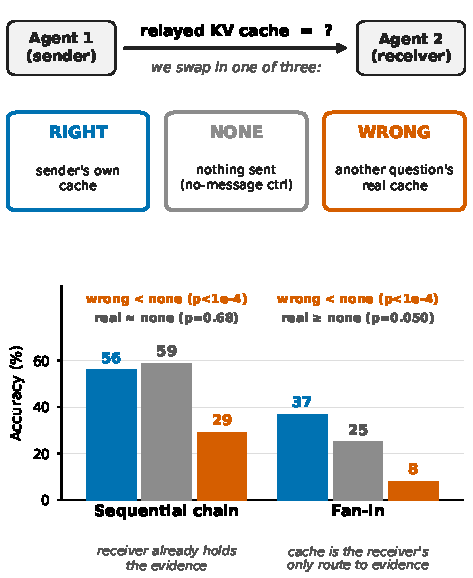
\includegraphics[width=\columnwidth]{figures/fig1_wrong_vs_none.pdf}
\caption{\textbf{Takeaway: a wrong cache is worse than no cache in both
topologies, but the right cache only clearly beats no cache when it is
the receiver's sole route to the evidence.} We replace the KV cache one
agent relays to the next with the right one, nothing (a no-message
control), or another question's real cache. Qwen2.5-7B-Instruct, HotpotQA,
$n{=}100$; exact paired McNemar tests, uncorrected. Mistral-7B shows the
same wrong-below-none gap in the chain (Table~\ref{tab:no_relay}).}
\label{fig:headline}
\end{figure}

\section{Introduction}

Language is how LLM agents normally talk to each other, and it is
expensive: every message must be re-encoded from scratch by its reader.
A growing line of work therefore relays the sender's key--value (KV)
cache instead of its words, so the receiver attends over the sender's
computed state directly \citep{kvcomm2025,latentmas2026}. These systems
rest on an assumption that is rarely tested: that the receiver uses the
specific content it is handed.

Testing that assumption takes a causal intervention. The standard audit
\citep{latentcommpay2026} swaps the relayed cache for zeros, moment-matched
noise, or another question's cache, and checks that accuracy falls. Those
controls still relay \emph{something}, so by themselves they cannot say
whether a wrong cache actively misleads the receiver or merely fails to
help. Zhang and Emu \citep{zhangemu2026} close this gap with a no-message
baseline and an ``other-message effect'' measured against it, and find
the effect is mixed: harmful on Qwen3-4B GSM8K, helpful on Qwen3-8B and
on MATH-500. That leaves open how general the effect is. Does it hold for
KV relay on multi-hop QA and across model families, and what decides
whether it is negative, and whether the right cache helps at all? The
question matters because if the receiver can get the evidence another way,
relay may be redundant when it is right and harmful when it is wrong.

We study these questions for KV relay. Following \citet{zhangemu2026} we
include a \textbf{dropped} condition, where the receiver is given its own
prompt and no cache at all (Figure~\ref{fig:headline}), and compare
\emph{right} (real), \emph{none} (dropped) and \emph{wrong} (mismatched, a
real cache from a different question). This separates three outcomes: a
cache that helps, a cache that is ignored, and a cache that misleads. We
run the comparison in three multi-agent topologies, a sequential chain, a
static fan-in, and a model-driven delegation loop, on Qwen2.5-7B-Instruct,
Mistral-7B-Instruct-v0.3 and Qwen3-8B, mainly on HotpotQA
\citep{hotpotqa2018}. Our central finding is that
\textbf{a wrong cache can be worse than no cache, while the value of the
right cache depends on whether it is the receiver's only route to the
evidence}:

\begin{itemize}[leftmargin=*,itemsep=1pt,topsep=2pt]
\item \textbf{Wrong is worse than none.} Mismatched caches score far
below dropped on Qwen2.5 (29.0\% vs.\ 59.0\%) and Mistral (16.0\% vs.\
48.0\%), both $p<0.001$, and in the fan-in (8.0\% vs.\ 25.0\%,
$p<0.0001$).
\item \textbf{Right versus none depends on topology.} In the chain the
right cache is not distinguishable from none on any model
($p=0.29$--$0.68$). In the fan-in it is better (37.0\% vs.\ 25.0\%,
$p=0.050$, borderline), where the cache is the aggregator's only source
of evidence.
\item \textbf{Content sensitivity is model-dependent.} On Qwen3-8B
(non-thinking mode), mismatched and dropped produce the identical output
on 45 of 50 examples.
\item \textbf{Compression does not erase the gap.} 8-bit and 4-bit
relays keep the same real-versus-mismatched gap as uncompressed relay.
\end{itemize}

We make no claim that KV relay improves accuracy or latency over text
relay or a single agent; our evaluation is single-GPU, uses $n{=}50$--$100$
per condition, and is mostly HotpotQA. Our contributions are:
\textbf{(1)} the first measurement, to our knowledge, of the no-message
comparison for KV relay across three topologies (chain, fan-in, model-driven
delegation) and three model families, extending the other-message effect
of \citet{zhangemu2026} beyond Qwen3 math and science tasks;
\textbf{(2)} evidence that a wrong cache is far worse than none on two of
three models and in two topologies, with a topology account of when the
right cache matters, an axis \citet{zhangemu2026} do not vary; and
\textbf{(3)} qualifying results we report rather than omit: a model with
no detected content sensitivity, a delegation loop where the effect is
attenuated, and compressed relays that preserve the gap.

\section{Related Work}
\label{sec:related}

\paragraph{Relaying state instead of text.} KVCOMM \citep{kvcomm2025}
corrects KV-cache offset drift when reusing cache across prefixes, and
LatentMAS \citep{latentmas2026} lets agents exchange latent ``thoughts''
through KV working memory; KVComm \citep{shikvcomm2025} is a distinct
system with a near-identical name. Recursive Language Models
\citep{rlm2026} let a root model delegate through a sandboxed REPL
rather than a fixed topology, and CanonicalMerge
\citep{canonicalmerge2026} studies merging parallel caches, reporting
downstream accuracy only. None of these tests whether the relayed
content is causally necessary.

\paragraph{Auditing whether relay carries content.} Cheng et al.\
\citep{latentcommpay2026} audit three published relay systems with
zeroed, moment-matched random and deranged (mismatched) substitution and
find content-specificity is system-dependent; their no-communication
control is a zeroed cache rather than an empty one. Zhang and Emu
\citep{zhangemu2026} audit latent channels, including KV caches, on
Qwen3-4B/8B with GSM8K, ARC-Challenge and MATH-500; they include a
no-message baseline and define an other-message effect against it, and
report mixed signs that reverse between model sizes. Brito and Baquero
\citep{latentagentslie2026} audit cache integrity under an adversarial
agent. We adopt the substitution methodology and the no-message
comparison, and extend them in three ways neither prior audit covers:
three topologies, including one the model constructs itself; a second
model family and multi-hop QA, where the other-message effect is strongly
negative on two of three models; and compressed relays. Our Qwen3-8B
result parallels the system and model-size dependence both papers report
(Appendix~\ref{app:relwork}).

\paragraph{KV compression and layer selection.} Quantization and layer
dropping shrink the relayed cache. KIVI \citep{kivi2024}, RotateKV
\citep{rotatekv2025} and KVQuant \citep{kvquant2024} identify the
difficulty of quantizing post-RoPE keys, which we confirm when a
rotation-based scheme in the style of TurboQuant \citep{turboquant2026}
and PolarQuant \citep{polarquant2026} fails on our pipeline
(Appendix~\ref{app:rotation}). ``No Free Swap'' \citep{nofreeswap2026}
finds layer redundancy depends on model and protocol, consistent with
our layer-selection results (Section~\ref{sec:results}). We use these
techniques only to test whether the causal finding survives compression;
further related work is in Appendix~\ref{app:relwork}.

\section{Audit Design}
\label{sec:method}

\paragraph{Conditions.} At the point a cache would be relayed we
substitute one of five contents (Table~\ref{tab:conditions}). Zeroed and
random are out-of-distribution sanity floors. \emph{Mismatched} and
\emph{dropped} are the informative pair: a mismatched cache is exactly as
valid a tensor as the real one, and dropped says whether wrong content is
worse than having none. Donor caches come from a pool of 20 held-out
questions never among the scored set, with one donor draw per scored
example. In every condition the receiver's prompt is unchanged, so only
the cache varies; this makes the prompt's statement that prior content is
in context literally false under dropped, a choice that works against,
not for, our finding that wrong is worse than none.

\begin{table}[t]
\centering
\small
\caption{What the receiver's cache holds under each condition.}
\label{tab:conditions}
\begin{tabular}{lp{5.2cm}}
\toprule
\textbf{Condition} & \textbf{Cache the receiver attends over} \\
\midrule
real       & the sender's own cache \\
dropped    & none: the receiver's own prompt only \\
zeroed     & all-zero tensors, same shape \\
random     & noise matching each tensor's mean and std \\
mismatched & a real cache from a different held-out question \\
\bottomrule
\end{tabular}
\end{table}

\paragraph{Topologies (Figure~\ref{fig:topologies}).} The \textbf{sequential chain} is a three-agent
pipeline (Reasoner, Verifier, Finalizer) in which each downstream agent's
prompt already contains the source passages. In the \textbf{fan-in}, the
ten HotpotQA passages are split across two child agents; their
RoPE-shifted caches are concatenated, and the aggregator sees only the
question plus the merged cache, with no independent copy of the passages.
In the \textbf{model-driven delegation loop} (RLM+KV), a root model writes
code in a sandboxed REPL and decides what to delegate; a sub-call's cache
is RoPE-shifted and spliced onto the root's, and the root keeps direct
access to the passages. No agent framework exposes KV cache as a
channel, so all three are built directly on \texttt{transformers}
\citep{transformers2020} (Appendix~\ref{app:method-ext}).

\begin{figure*}[t]
\centering
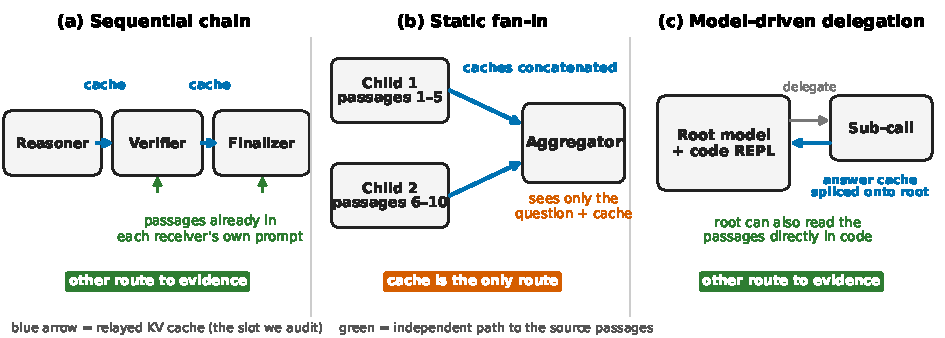
\includegraphics[width=0.92\textwidth]{figures/fig2_topologies.pdf}
\caption{\textbf{Takeaway: the three topologies differ in whether the
receiver has any route to the evidence other than the relayed cache, which
is the variable our results turn on.} Blue arrows are the relayed KV cache
we substitute; green marks an independent path to the source passages. In
the chain the receiver's own prompt already contains the passages; in the
fan-in the aggregator sees only the question and the merged caches; in the
delegation loop the root can read the passages directly in code.}
\label{fig:topologies}
\end{figure*}

\paragraph{Implementation.} Every configuration shares the same
Reasoner, Verifier and Finalizer prompts as a text-relay baseline that
passes decoded text instead of cache, so differences between relay
variants are attributable to the relayed content, not to prompt wording.
All decode paths use the same repetition penalty (1.05) and the
\texttt{sdpa} attention backend. Quantized and layer-selected variants
(8-bit and 4-bit per-head or per-channel min--max quantization; dropping
calibration-identified low-importance layers with zero reconstruction) are
audited with the same five conditions.

\paragraph{Models and data.} Qwen2.5-7B-Instruct \citep{qwen2p5_2024} is
the primary model in all three topologies. Mistral-7B-Instruct-v0.3
\citep{mistral7b2023} and Qwen3-8B \citep{qwen3_2025} (non-thinking mode)
run the chain only. We use HotpotQA (distractor setting) with a GSM8K
\citep{gsm8k2021} and a 2WikiMultihopQA replication in
Appendix~\ref{app:results-ext}. All runs use bf16, greedy decoding and one
RTX 4090.

\paragraph{Statistics.} We report accuracy (exact match) and token F1,
exact paired McNemar tests on per-example correctness, and paired
bootstrap 95\% CIs (10{,}000 resamples) on F1 differences. We designate
eight primary comparisons (real vs.\ mismatched and dropped vs.\
mismatched, per model and topology) and Holm-adjust them
(Appendix~\ref{app:stats}); the family was fixed after the initial
$n{=}50$ runs, and the two Qwen2.5 legs that were weakest were then
re-run at $n{=}100$, which we disclose as a form of optional stopping.
Every other $p$-value is descriptive and uncorrected.

\section{Results}
\label{sec:results}

\subsection{Sequential chain: wrong is worse than none}

\paragraph{Content matters at all.} On the uncompressed chain
(config \texttt{A}, Qwen2.5, $n{=}50$), real scores 50.0/64.0
(accuracy/F1) against 0.0/0.0 for zeroed and random and 28.0/37.1 for
mismatched; real beats zeroed and random at $p<0.0001$ and mismatched at
$p=0.0127$ (Table~\ref{tab:ladder}). The same ordering holds for the
compressed and layer-selected configurations (Appendix
Table~\ref{tab:causal_audit_full}) and replicates on a second task and
dataset: on GSM8K, real scores 90.0\% against 0.0\% zeroed, 2.0\% random and
28.0\% mismatched (all $p<0.0001$), and on 2WikiMultihopQA 54.0/62.5 against
0.0/0.7, 0.0/0.0 and 16.0/23.4 (real vs.\ mismatched $p=0.000004$, 19 of 19
discordant pairs favoring real).

\begin{table*}[t]
\centering
\small
\caption{The zeroed / random / mismatched ladder on config \texttt{A} (and the
fan-in and delegation topologies), accuracy / F1 (\%), $n{=}50$. Real beats
zeroed and random at $p<0.0001$ in every row except Qwen3-8B and the
delegation loop, where a direct path to the passages keeps zeroed and random
above zero. GSM8K reports accuracy only. $^\dagger$Non-thinking mode.}
\label{tab:ladder}
\begin{tabular}{lccccc}
\toprule
\textbf{Model, task, topology} & \textcolor{realblue}{\textbf{Real}} & \textbf{Zeroed} & \textbf{Random} & \textcolor{wrongred}{\textbf{Mismatched}} & $p$(Real, Mism.) \\
\midrule
Qwen2.5-7B, HotpotQA, chain       & 50.0/64.0 & 0.0/0.0   & 0.0/0.0 & 28.0/37.1 & 0.0127 \\
Mistral-7B, HotpotQA, chain       & 56.0/63.3 & 0.0/0.5   & 0.0/0.3 & 16.0/26.4 & 0.000011 \\
Qwen3-8B, HotpotQA, chain$^\dagger$ & 54.0/67.2 & 46.0/55.8 & 0.0/0.0 & 64.0/74.8 & 0.30 \\
Qwen2.5-7B, GSM8K, chain          & 90.0/--- & 0.0/---   & 2.0/--- & 28.0/---  & $<$0.0001 \\
Qwen2.5-7B, 2Wiki, chain          & 54.0/62.5 & 0.0/0.7   & 0.0/0.0 & 16.0/23.4 & 0.000004 \\
Qwen2.5-7B, HotpotQA, fan-in      & 40.0/53.0 & 0.0/0.8   & 0.0/0.0 & 6.0/12.0  & 0.0001 \\
Qwen2.5-7B, HotpotQA, delegation  & 24.0/32.3 & 8.0/11.2  & 6.0/9.2 & 10.0/15.5 & 0.0156 \\
\bottomrule
\end{tabular}
\end{table*}

\begin{table*}[t]
\centering
\small
\caption{Dropped (no-relay) control. Accuracy / F1 (\%) per condition; exact
paired McNemar $p$-values, uncorrected (Holm-adjusted values for the
primary family are in Appendix~\ref{app:stats}). Qwen2.5 rows are $n{=}100$,
others $n{=}50$. $^\dagger$Qwen3-8B ran with thinking disabled, so an
architecture effect cannot be separated from a decoding-mode effect.}
\label{tab:no_relay}
\begin{tabular}{lccccccc}
\toprule
 & \multicolumn{3}{c}{\textbf{Accuracy / F1}} & \multicolumn{3}{c}{\textbf{$p$-value}} & \\
\cmidrule(lr){2-4}\cmidrule(lr){5-7}
\textbf{Model / topology} & \textcolor{realblue}{\textbf{Real}} & \textbf{Dropped} & \textcolor{wrongred}{\textbf{Mismatched}} & Real\,/\,Dropped & Real\,/\,Mism. & Dropped\,/\,Mism. & $n$ \\
\midrule
Qwen2.5-7B, chain        & 56.0/69.1 & 59.0/69.0 & 29.0/40.6 & 0.68  & 0.000025 & $<$0.0001 & 100 \\
Mistral-7B, chain        & 56.0/63.3 & 48.0/58.4 & 16.0/26.4 & 0.29  & 0.000011 & 0.0004    & 50 \\
Qwen3-8B, chain$^\dagger$& 54.0/67.2 & 62.0/71.4 & 64.0/74.8 & 0.42  & 0.30     & 1.0       & 50 \\
\midrule
Qwen2.5-7B, fan-in       & 37.0/46.6 & 25.0/33.4 & 8.0/13.0  & 0.050 & $<$0.0001 & 0.000076 & 100 \\
\bottomrule
\end{tabular}
\end{table*}

\paragraph{Wrong is worse than none.} Table~\ref{tab:no_relay} shows the
central result. On Qwen2.5 and Mistral, a mismatched cache is worse than
no relay ($p<0.0001$ and $p=0.0004$) and worse than the right cache
($p=0.000025$ and $p=0.000011$): wrong content is not merely unhelpful,
it is actively harmful relative to having none. Manual review of 20 of the
36 wrong mismatched answers finds donor-question content leaking into the
output only rarely (one clear case; Appendix~\ref{app:results-ext}), so
the harm is mostly confusion on the real question rather than topic
substitution.

\paragraph{Right is not distinguishable from none.} The right cache does
not beat dropped on any model: $p=0.68$ (Qwen2.5), $0.29$ (Mistral) and
$0.42$ (Qwen3-8B), with the point estimate pointing in different
directions across models. Doubling Qwen2.5's sample from $50$ to $100$
moved the estimate toward zero, not away from it (56.0\% vs.\ 59.0\%, F1
difference $+0.1$, 95\% CI $[-8.2,+8.4]$). We read this as
indistinguishable at this sample size, not as evidence that the cache is
unnecessary or that the two are equivalent. In line with this, a single
agent with no relay (57.0/68.4) and the full relay chain (56.0/69.1) score
similarly (Appendix Table~\ref{tab:full}); we ran no paired test between
them.

\paragraph{What we ruled out.} Before trusting these numbers we checked
the failure modes a skeptical reader would raise. Donor leakage: every
mismatched donor question was compared with its scored question directly,
with no overlap. Garbled output as a scoring artifact: a garbage-signature
scan over fan-in generations flags 0/50 real, 4/50 mismatched, 23/50
zeroed and 48/50 random outputs, a monotone ordering matching accuracy, with
random noise more degraded than zeros (a zero key is weak and can be
down-weighted, while realistic noise resembles signal and misdirects
attention). Decoding confound: Qwen's own default repetition penalty is our
setting (1.05) and Mistral's specifies none, so our setting corrects
\emph{more} for Mistral, the opposite of what an unfair-to-Mistral confound
needs. Reproducibility: greedy decoding is bit-identical across reruns in
the chain and fan-in, and in the delegation loop after our determinism fix.

\subsection{Fan-in: when the cache is the only route}

In the fan-in the picture changes. Dropped falls to 25.0/33.4, well below
real (37.0/46.6), because the aggregator has no other copy of the
passages. Real versus dropped is borderline ($p=0.050$, F1 difference
$+13.2$, 95\% CI $[+2.2,+24.2]$, which excludes zero); at $n{=}50$ it was
$p=0.12$. Real decisively beats mismatched ($p<0.0001$, 30 of 31
discordant pairs), and dropped still beats mismatched ($p=0.000076$, 18
of 19 discordant pairs): even where the cache is the only route to the
evidence, a wrong one is worse than none. At $n{=}50$ the full ladder is
clean: real 40.0/53.0, zeroed 0.0/0.8, random 0.0/0.0, mismatched
6.0/12.0 (real vs.\ mismatched $p=0.0001$).

\paragraph{Why the two topologies differ.} We propose that the chain's
receiver already holds the passages in its own prompt, so a wrong cache
acts as interference with information it has, while the fan-in's
aggregator depends on the cache for the evidence. This explanation fits
the data but is not isolated by a controlled ablation, since the two
topologies differ in more than passage access (Limitations).

\subsection{Model-driven delegation}

The RLM+KV loop is the least favorable topology for a clean result: our
HotpotQA questions do not need decomposition, and the root can read the
passages directly. Accuracy of \texttt{kv} against \texttt{text} relay is
unresolved at $n{=}50$ (24.0/32.3 vs.\ 22.0/28.5, $p=1.0$), and we claim
no KV accuracy win. The audit still resolves: \texttt{kv} beats zeroed
($p=0.0078$), random ($p=0.0039$) and mismatched ($p=0.0156$), with F1
differences of $+0.210$, $+0.230$ and $+0.167$ (all CIs exclude zero).
Zeroed and random land at 8.0\% and 6.0\% rather than near zero because
the root's direct path to the passages bypasses the audited channel, so
this audit is narrower than the other two. The dropped control here is
directionally consistent but not significant (\texttt{kv} vs.\ dropped
$p=0.22$; dropped vs.\ mismatched $p=0.25$, 3 of 3 discordant pairs favor
dropped). Whether a session finishes within its turn budget tracks the
same ordering and resolves the leg accuracy cannot: the share of sessions
that time out is 22\% for real, 42\% for mismatched, 72\% for zeroed and 76\%
for random, with every pairwise difference significant, including mismatched
vs.\ random ($p<0.0001$; Appendix~\ref{app:behavioral}). The prototype is
bit-identically reproducible under our determinism fix
(Appendix~\ref{app:nondeterminism}).

\subsection{Architecture dependence}

\paragraph{Qwen3-8B shows no detected content sensitivity.} Random still
collapses accuracy ($p<0.0001$), but real is indistinguishable from
zeroed and mismatched ($p=0.30$--$0.79$ across four comparisons on configurations \texttt{A} and \texttt{D}), and
mismatched and dropped give the identical output string on 45 of 50
examples. The right cache changes about 44\% of outputs relative to
dropped, with no net accuracy change (54.0\% real, 62.0\% dropped, 64.0\%
mismatched; no pairwise comparison significant). We checked this is not a
bug (no donor leakage, selective substitution; Appendix~\ref{app:qwen3}).
It is consistent with robustness to irrelevant context but, because the
run used non-thinking mode, we cannot separate an architecture effect from
a decoding-mode effect.

\paragraph{Layer selection is also architecture-dependent.} Dropping a
near-identical share of layers costs 30.5 F1 points on Mistral
($p=0.0001$) but a smaller, not significant amount on Qwen2.5 ($p=0.34$)
and nothing detectable on Qwen3-8B ($p=1.0$). Mistral's failures are also
different in kind: fabricated tangents and repetition loops, not the short
near-misses typical of Qwen (Appendix~\ref{app:failurechar}). On Mistral,
layer-selected configurations \texttt{C} and \texttt{D} show an attenuated
real-versus-mismatched gap ($p=0.51$, $0.375$), which tracks their
degraded baseline, whereas quantization-only configurations show the full
gap.

\subsection{Compression does not make the cache generic}

If the cache carried only generic state, compressing it should not matter;
if it is content-specific, compression should leave the real-versus-
mismatched gap intact. It does. \texttt{B\_int8} and \texttt{B\_int4\_kivi}
keep the gap on Qwen2.5 and Mistral (Appendix
Table~\ref{tab:causal_audit_full}; Qwen2.5 real vs.\ mismatched
$p\le0.02$ for all four compressed configurations). \texttt{B\_int8} is
indistinguishable from uncompressed relay ($p=1.0$, 3 discordant of 100)
at 2.00$\times$ smaller. Uniform 4-bit quantization collapses to 0.0/0.0,
traced to keys being cached after RoPE; quantizing keys per channel
(KIVI-style, \texttt{B\_int4\_kivi}) recovers 52.0/64.1 at 3.96$\times$
compression. That ratio comes from a packing-enabled compressor applied
after the accuracy was measured on the unpacked version; packing is
verified bit-identical on tensors but we did not re-run the full pipeline
(Appendix~\ref{app:nibble}). An anchor-based offset-correction baseline
fails outright (Appendix~\ref{app:limitations}). We report compressed
bytes and make no latency claim: nothing is transmitted over a network and
every layer still runs.

\begin{table}[t]
\centering
\small
\caption{Compression on the uncompressed-relay chain, Qwen2.5-7B-Instruct,
HotpotQA, $n{=}100$. Ratios are relative to \texttt{A}'s 144.35~MB per hop;
latency and no-relay baselines are in Table~\ref{tab:full}.}
\label{tab:main}
\begin{tabular}{lcc}
\toprule
\textbf{Config} & \textbf{Acc.\ / F1} & \textbf{KV/hop} \\
\midrule
A & 56.0 / 69.1 & 144.35 MB \\
B\_int8 & 57.0 / 70.5 & 72.16 MB (2.00x) \\
B\_int4 & 0.0 / 0.0 & 38.38 MB (4.00x) \\
\textbf{B\_int4\_kivi} & \textbf{52.0 / 64.1} & 36.43 MB (3.96x) \\
C & 43.0 / 57.8 & 104.16 MB \\
D & 50.0 / 61.9 & 37.82 MB (3.82x) \\
E & 9.0 / 17.4 & 35.63 MB \\
\bottomrule
\end{tabular}
\end{table}

\section{Discussion}

\paragraph{For system designers.} Audit a relay channel against silence,
not only against noise. A misrouted or stale cache is a worse failure than
no relay, so where the integrity of a cache cannot be guaranteed, dropping
it is the safer fallback, though not a free one where the cache is the
receiver's only route (the fan-in).

\paragraph{When the right cache matters.} The right cache clearly helps
only where it carries evidence the receiver cannot get elsewhere. The
delegation loop, where the root keeps its own path to the passages,
shows the weakest effects, as this account predicts.

\paragraph{Per-model audits.} Qwen3-8B's insensitivity shows that content
dependence is not visible from one architecture alone, so a relay or
compression recipe validated on one model should be re-audited on the
next. This agrees with Zhang and Emu's finding that the sign of the
other-message effect reverses between Qwen3 sizes \citep{zhangemu2026}.

\section{Conclusion}

Measuring the no-message comparison for KV relay across three topologies and
three models, we found that a wrong cache can be worse than no cache, while
the right cache's value depends on whether it is the receiver's only route
to the evidence.
This matters to anyone building agent systems around a KV channel: audit
against silence, and treat a misrouted cache as a failure worse than
dropping relay. The result holds on two of three models and two of three
topologies tested, mostly on HotpotQA, and we do not claim more.

\section*{Limitations}
\label{sec:limitations}

\begin{itemize}[leftmargin=*,itemsep=1pt]
\item \textbf{Mechanism not isolated.} The explanation for the chain and
fan-in difference (passage access) is a hypothesis; the topologies also
differ in other ways, and we ran no ablation that changes passage access
alone.
\item \textbf{No text-relay control for wrong content.} We did not relay
a different question's decoded \emph{text} in the same slot, so we cannot
say whether the harm is specific to KV or is ordinary distractor harm.
\item \textbf{Receiver necessity is topology-specific.} Whether the
receiver needs the cache has no single answer, and we do not average the
chain and fan-in into one.
\item \textbf{Prompt premise.} Receiver prompts assert that prior content
is in context, which is false under dropped; we kept prompts identical so
only the cache differs.
\item \textbf{Sample size and donors.} Most comparisons use $n{=}50$ with
one donor draw per example for mismatched, and several comparisons remain
underpowered rather than confirmed null; the two Qwen2.5 legs extended to
$n{=}100$ were extended after seeing initial results.
\item \textbf{Scope.} Mostly HotpotQA with Qwen2.5-7B; Mistral and
Qwen3-8B on the chain only, Qwen3-8B in non-thinking mode only; greedy
decoding only; one dataset replication each for GSM8K and
2WikiMultihopQA; no mixed-architecture relay within one pipeline.
\item \textbf{No latency or systems claim.} Single process, single GPU,
no network transfer; compressed-byte accounting reflects what a
distributed deployment would send, and smaller caches were not faster.
\item \textbf{Compression accounting.} Accuracy for 4-bit configurations
was measured before nibble packing was implemented; only the compression
ratios reflect packing.
\item \textbf{Exploratory review.} The donor-content leakage review is a
single-annotator, manual observation on a subset.
\end{itemize}

\section*{Use of AI Assistants}

An AI coding and writing assistant (Claude Code) was used for code
development and editing assistance. The authors designed the study, ran
all experiments, and verified every reported result.

\bibliography{references_v6}
\bibliographystyle{acl_natbib}


\appendix

\section{Statistical Details}
\label{app:stats}

\paragraph{Primary comparisons.} We designate eight comparisons as primary:
real vs.\ mismatched and dropped vs.\ mismatched, for each of Qwen2.5 chain,
Qwen2.5 fan-in, Mistral chain and Qwen3-8B chain. The family was fixed after
the initial $n{=}50$ runs. Holm-adjusted $p$-values (unadjusted $\to$
adjusted): Qwen2.5 fan-in real vs.\ mismatched $3.0\times10^{-8}\to
2.4\times10^{-7}$; Qwen2.5 chain dropped vs.\ mismatched $6.9\times10^{-8}\to
4.9\times10^{-7}$; Mistral chain real vs.\ mismatched $1.1\times10^{-5}\to
6.6\times10^{-5}$; Qwen2.5 chain real vs.\ mismatched $2.5\times10^{-5}\to
1.3\times10^{-4}$; Qwen2.5 fan-in dropped vs.\ mismatched $7.6\times10^{-5}\to
3.0\times10^{-4}$; Mistral chain dropped vs.\ mismatched $4\times10^{-4}\to
1.2\times10^{-3}$; Qwen3-8B chain real vs.\ mismatched $0.30\to0.60$; Qwen3-8B
chain dropped vs.\ mismatched $1.0\to1.0$. Every primary comparison that was
significant before correction stays significant after it.

\paragraph{Optional stopping.} After the initial $n{=}50$ runs, the Qwen2.5
chain and fan-in were re-run at $n{=}100$ to add power to the two weakest legs
(real vs.\ dropped in each topology). The $n{=}100$ sets contain the original
$n{=}50$ examples, so the two sizes are not independent. The two
dropped-versus-mismatched comparisons in these rows were already significant
at $n{=}50$ and strengthened at $n{=}100$. All non-primary $p$-values,
including every zeroed and random leg, cross-model layer-selection cost and
compression comparison, are descriptive and uncorrected.

\paragraph{Mismatched donors.} Donor caches are drawn from a pool of 20
held-out questions, confirmed disjoint from the scored set by direct
question-text comparison. Each scored example uses one donor assignment, which
is not resampled across conditions.

\section{Full Causal-Audit Table}
\label{app:tables}

% Appendix table: every real/zeroed/random/mismatched comparison (accuracy/F1, %).
% Numbers unchanged from table_causal_audit_full.tex; caption rewritten for the paper.
\begin{table*}[t]
\centering
\small
\caption{Every real / zeroed / random / mismatched audit in this paper, as accuracy / F1 (\%). The dropped control is reported separately in Table~\ref{tab:no_relay}. Real vs.\ zeroed and vs.\ random is significant ($p<0.0001$, exact McNemar) in every row except Qwen3-8B, where content sensitivity is itself weak (Section~\ref{sec:results}). Real vs.\ mismatched is significant in every row except Mistral \texttt{C}/\texttt{D} (a heavily degraded layer-selection baseline leaves little headroom) and Qwen3-8B. GSM8K reports accuracy only.}
\label{tab:causal_audit_full}
\begin{tabular}{llccccc}
\toprule
\textbf{Config} & \textbf{Model / task / topology} & \textbf{Real} & \textbf{Zeroed} & \textbf{Random} & \textbf{Mismatched} & \textbf{$n$} \\
\midrule
\multicolumn{7}{l}{\emph{Qwen2.5-7B-Instruct, HotpotQA, sequential chain}} \\
A            & ---                         & 50.0/64.0 & 0.0/0.0  & 0.0/0.0  & 28.0/37.1 & 50 \\
D            & ---                         & 54.0/60.2 & 0.0/0.0  & 0.0/0.2  & 26.0/32.2 & 50 \\
B\_int8      & ---                         & 54.0/68.0 & 0.0/0.0  & 0.0/0.0  & 24.0/34.4 & 50 \\
C            & ---                         & 46.0/55.7 & 0.0/0.0  & 0.0/0.0  & 24.0/38.9 & 50 \\
B\_int4\_kivi& ---                         & 50.0/61.7 & 0.0/0.0  & 0.0/0.0  & 28.0/34.7 & 50 \\
\midrule
\multicolumn{7}{l}{\emph{Other models, tasks and topologies}} \\
A            & Mistral-7B-Instruct-v0.3    & 56.0/63.3 & 0.0/0.5  & 0.0/0.3  & 16.0/26.4 & 50 \\
C            & Mistral-7B-Instruct-v0.3    & 20.0/30.3 & 0.0/0.5  & 0.0/0.1  & 14.0/26.1 & 50 \\
D            & Mistral-7B-Instruct-v0.3    & 22.0/32.8 & 0.0/0.5  & 0.0/0.1  & 16.0/29.3 & 50 \\
B\_int8      & Mistral-7B-Instruct-v0.3    & 56.0/63.3 & 0.0/0.5  & 0.0/0.1  & 20.0/29.3 & 50 \\
B\_int4\_kivi& Mistral-7B-Instruct-v0.3    & 54.0/63.2 & 0.0/0.5  & 0.0/0.1  & 16.0/25.0 & 50 \\
A            & Qwen3-8B (non-thinking)     & 54.0/67.2 & 46.0/55.8& 0.0/0.0  & 64.0/74.8 & 50 \\
D            & Qwen3-8B (non-thinking)     & 56.0/71.2 & 46.0/55.8& 2.0/5.0  & 52.0/62.4 & 50 \\
A            & GSM8K (Qwen2.5)             & 90.0/---  & 0.0/---  & 2.0/---  & 28.0/---  & 50 \\
A            & 2WikiMultihopQA (Qwen2.5)   & 54.0/62.5 & 0.0/0.7  & 0.0/0.0  & 16.0/23.4 & 50 \\
kv (fan-in)  & Fan-in (Qwen2.5)            & 40.0/53.0 & 0.0/0.8  & 0.0/0.0  & 6.0/12.0  & 50 \\
kv (RLM+KV)  & Model-driven delegation (Qwen2.5) & 24.0/32.3 & 8.0/11.2 & 6.0/9.2  & 10.0/15.5 & 50 \\
\bottomrule
\end{tabular}
\end{table*}


\section{Extended Related Work}
\label{app:relwork}

\paragraph{Rotation-based quantization.}
\label{app:rotation}
We applied a fixed orthonormal
Hadamard rotation to both keys and values before quantizing
(covering PolarQuant's \citep{polarquant2026} rotate-then-quantize
step, not TurboQuant's \citep{turboquant2026} separate QJL
bias-correction term; these are two distinct papers sharing only two
authors, not one work under two names). On our model this produced
severely out-of-distribution decoded output. We traced this to keys'
RoPE encoding: K is cached after RoPE is applied, which mixes channel
pairs by a position-dependent phase, and a second, RoPE-agnostic
rotation disrupts that structure. KIVI \citep{kivi2024} quantizes keys
per-channel and values per-token, motivated by RoPE leaving channel-wise
magnitude more consistent across positions than per-head ranges assume.
RotateKV \citep{rotatekv2025} instead rotates \emph{before} RoPE via
Pre-RoPE Grouped-Head Rotation, explicitly designed to avoid this
interaction. KVQuant \citep{kvquant2024} similarly identifies post-RoPE
key quantization as harder than value quantization for the same reason.

\paragraph{Considered but not adopted compression strategies.}
Orthogonal Backfill \citep{orthobackfill2026} injects a low-rank
residual of discarded content orthogonal to what is retained; its
published formula requires attention weights our \texttt{sdpa} decode
path does not expose, and given our own evidence that naive
reproductions can actively mislead, we did not ship an approximated
version. KVTC \citep{kvtc2026} applies media-compression-style
transform coding (PCA decorrelation, adaptive quantization, entropy
coding) for up to 20x compression, a third paradigm distinct from
uniform quantization and rotation; NVIDIA's kvpress library and
TensorRT-LLM's reuse-aware cache confirm KV compression is an actively
contested axis of deployed systems.

\paragraph{Cheng et al.\ and system-dependence.} Cheng et al.\
\citep{latentcommpay2026} find content-specificity is
\emph{system}-dependent: ceiling effect on LatentMAS, partial on
KVComm, no detected advantage on C2C, holding audit methodology fixed
and varying which published relay system is tested. Our Qwen3-8B
extension independently arrives at the same qualitative pattern while
holding the relay mechanism fixed and varying the model instead. Two
audits converging on ``it depends, and not on accuracy alone'' from
different varied axes is more informative than either alone. ``When KV
Cache Reuse Fails in Multi-Agent Systems'' \citep{kvreusefails2026}
shows reuse strategies effective for generation agents can silently
corrupt an LLM judge's cross-candidate comparison, a complementary
critical-auditing result we do not directly test.

\paragraph{CanonicalMerge.} \citep{canonicalmerge2026} is close to our
fan-in topology: near-identical models (Qwen3-1.7B/4B versus our
Qwen2.5-7B-Instruct/Mistral-7B-Instruct-v0.3) and a closely related task
(HotpotQA bridge questions versus our full distractor HotpotQA),
addressing a real question we do not (whether merge order biases the
result) but reporting only downstream accuracy, with no
causal-intervention test of whether merged content is specifically, not
just numerously, necessary.

\paragraph{AdaK and Pitfalls of KV Cache Compression.} AdaK
\citep{adak2026} reports adaptive KV-budget estimation generalizing
across Qwen3 (4B/8B) and Mistral-7B-Instruct-v0.2, the same two
architecture families we test (not a third; Llama is not among AdaK's
evaluated models despite a superficial reading suggesting otherwise),
which looks like a counterexample to our architecture-dependence claim.
We do not believe it is: AdaK estimates budget per-instance and
per-model at inference time rather than committing to one
calibration-time ranking applied uniformly, so it never assumes a
fixed, transferable ranking is safe to act on; its success is a
positive instance of our principle, not a counterexample. This is our
reading of the mechanism, not a reimplementation we verified ourselves.
``The Pitfalls of KV Cache Compression'' \citep{pitfallskv2026} argues
compression methods optimize aggregate metrics while implicitly
equating token retention with functional preservation; our contribution
is a causally grounded, cross-axis demonstration of this within one
system (depth, position, content-identity) rather than the abstract
observation.

\section{Extended Method}
\label{app:method-ext}

\paragraph{Causal-audit baseline caveat.} Zero-ablation is a
known-imperfect causal baseline in the interpretability literature: it
pushes activations off the training distribution, which can produce
large behavioral changes unrelated to whether the zeroed content
carried meaningful information. We treat moment-matched-random and
mismatched, which preserve realistic statistics or substitute another
real cache, as the more informative evidence, and zero-ablation as a
supplementary sanity floor. A fully rigorous ``no difference'' claim
would use a pre-registered equivalence margin rather than absence of
significance; we did not have the budget to pre-register and power such
a test.

\paragraph{Why RLM+KV is implemented from scratch.} We implement the
RLM+KV loop directly on \texttt{transformers} \citep{transformers2020}
rather than \texttt{dspy.RLM}, the first-party DSPy implementation of
RLM. DSPy is built on \texttt{litellm} and is, by design, a text-only,
API-centric orchestration layer: a sub-call through \texttt{dspy.RLM}'s
\texttt{llm\_query} returns decoded text and nothing else, with no
exposure anywhere in the framework to a model's KV cache. Our
\texttt{kv} return channel is not implementable on top of it; we
verified this against DSPy's own documentation before committing to a
from-scratch implementation.

\section{Extended Results}
\label{app:results-ext}

\paragraph{Qualitative texture (sequential chain).} Mismatched's wrong
answers are coherent and grammatical, real linguistic structure
attached to the wrong question; zeroed produces garbled but
recognizable English; random is more degraded still (code-fragment
tokens, mixed-language noise) despite matching real activation
statistics. We read this as a zero vector being a weak attention key
that can be down-weighted, while realistic random noise resembles
genuine signal and actively misdirects attention. A fan-in
garbage-signature scan of all 200 generations gives the identical
texture: 0/50 flagged for real, 4/50 mismatched, 23/50 zeroed, 48/50
random.

\paragraph{Donor-content bleed-through, in full.} Manually reviewing 20
of 36 incorrect \texttt{A\_audit\_mismatched} answers against their
donor question: one unambiguous instance (a Kansas university
fight-song question produced ``Ellie Goulding,'' traceable only to a
donor question about that singer) and one weaker, ambiguous case; the
remainder show ordinary failure on the real question's own topic. One
annotator, no automated classifier or inter-annotator agreement check;
a rigorous version would classify the full set of incorrect examples
automatically or with multiple annotators, which we did not have the
budget to complete.

\paragraph{Layer-selection cost magnitude, full detail.} The
architecture-dependence claim in Section~\ref{sec:results} compares a
near-identical dropped-layer proportion: 9/32 layers (28\%) on Mistral
versus 8/28 layers (29\%) on Qwen2.5. Mistral's cost (30.5 F1 points,
$p=0.0001$) is confirmed significant; Qwen2.5's smaller cost is not yet
significant at $n=100$ ($p=0.34$), but the cross-model claim does not
rest on that reaching significance: even Qwen's most generous
uncertainty bound (F1 CI upper $+16.4$ points) is under half of
Mistral's confirmed collapse. Qwen3-8B's $D$-vs-$A$ comparison ($p=1.0$)
rests on only 3 discordant pairs out of 50, consistent with noise
rather than a real effect.

\paragraph{Mistral layer-selection, full explanation.} On \texttt{C},
mismatched beats zeroed/random ($p=0.0156$ each) but is not
distinguishable from real ($p=0.51$, F1 CI includes zero); \texttt{D}
shows the identical pattern ($p=0.0078$; $p=0.375$). Both track
\texttt{C}/\texttt{D}'s own degraded Mistral baseline (20.0\%/22.0\%
vs.\ Qwen's 46.0\%/50.0\%): less headroom to detect a further
real-vs-mismatched gap on an already-degraded baseline, not a failure
to replicate content-dependence. \texttt{B\_int8} on Mistral replicates
the full clean pattern, matching every quantization-only configuration;
layer-selection configurations show the attenuated pattern,
quantization-only configurations do not, consistently across two
separate experiments.

\paragraph{GSM8K confirmatory run.} $n=50$, Qwen2.5: \texttt{D} matched
\texttt{A}'s accuracy exactly (McNemar $p=1.0$, more decisively free
than on HotpotQA); the causal audit's three-tier ordering held with
every comparison significant ($p<0.0002$), larger effect sizes than the
original HotpotQA run. One run on one additional task, not a systematic
multi-task study; we did not extend \texttt{B\_int8}/\texttt{D}-family
audits or Mistral to GSM8K.

\paragraph{2WikiMultihopQA confirmatory run, verification detail.}
\label{app:2wiki}
All four conditions (\texttt{A} and its three audit variants) were
scored on the identical 50 paired examples, confirmed by matching
example index, question text, and gold answer across conditions. The
mismatched condition drew from a held-out donor pool of 20 distinct
questions; checking every donor question against all 50 scored
questions directly, none matched, and all 100 mismatched substitutions
(50 examples times two relay hops) were confirmed applied via the
per-example audit logs. Accuracy, F1, and latency were independently
reconstructed from the per-example records and matched the evaluator's
own summary exactly. Real versus mismatched had 19 discordant pairs,
all 19 favoring real and none favoring mismatched, F1 delta $+39.1$
points, 95\% bootstrap CI $[+26.1, +52.3]$. This is a single
confirmatory run on one additional dataset and one configuration, not a
systematic cross-dataset study.

\paragraph{Fan-in mismatched-vs-zeroed/random leg.} Not significant by
exact McNemar ($p=0.25$ each, 3 discordant pairs, the test's own floor
at that count), but the F1 bootstrap CI excludes zero for both
($+0.112$ [$+0.035,+0.200$], $+0.120$ [$+0.047,+0.206$]):
accuracy-level evidence is underpowered at this $n$ for this specific
leg while the finer-grained F1 comparison trends real.

\section{Qwen3-8B Verification}
\label{app:qwen3}

We verified the Qwen3-8B exception (Section~\ref{sec:results}) is a
real effect, not a bug, three ways: no donor-question pool leakage;
\texttt{A\_audit\_zeroed} and \texttt{D\_audit\_zeroed} produce
byte-identical output on all 50 examples, which looked alarming until
traced to \texttt{D}'s own \texttt{zeros} reconstruction strategy
composing correctly with the audit's own zeroing, not a bug; and real,
zeroed, and mismatched overlap on only 10--24 of 50 examples pairwise,
confirming the substitution takes effect selectively rather than being
silently inert. We do not have a mechanistic explanation for the
difference; we report it as an empirical observation and flag candidate
mechanisms as future work.

\section{RLM+KV Behavioral Signal}
\label{app:behavioral}

Timeout rate, mean turn count, and mean delegation-call count are
monotonic across conditions (real 22\% timeout, 7.72 turns, 1.38 calls;
mismatched 42\%/8.48/1.12; zeroed 72\%/9.46/0.76; random 76\%/9.60/0.66).
Substituting ``session finished without exhausting its turn budget''
for ``correct'' in the same paired McNemar test, every comparison is
significant, including mismatched versus random ($p<0.0001$), exactly
the leg final-answer accuracy left unresolved (real vs.\ mismatched
$p=0.0309$; real vs.\ zeroed/random $p<0.0001$ each; mismatched vs.\
zeroed $p=0.0001$). We verified this run shows no new degenerate output
at this scale (0/50 flagged for real/text; a clean, monotonic
3/50--48/50 ordering across the remaining conditions).

\section{RLM+KV Non-Determinism: Diagnosis and Fix}
\label{app:nondeterminism}

An earlier run of this experiment was not run-to-run deterministic.
Diffing raw generations for the identical 50 questions between two
independent runs under greedy decoding found 15 of 50 (30\%)
\texttt{text}-channel examples produced genuinely different output,
plausibly GPU floating-point non-associativity cascading through this
prototype's long, self-referential decode loop (unlike the two fixed
topologies, confirmed bit-identical across reruns). We fixed this by
forcing \texttt{torch.use\_deterministic\_algorithms(True,
warn\_only=True)} and setting \texttt{CUBLAS\_WORKSPACE\_CONFIG} before
any CUDA context exists. Verification: a rerun of the \texttt{text}
channel on 20 questions produced 0/20 differing raw answers against the
pre-fix run, including all 7 of the originally divergent examples. We
then reran the full five-channel, $n=50$ ladder and diffed every field,
not only the ones reported in Section~\ref{sec:results}: exact match,
F1, timeout rate, and delegation-call count are bit-identical across
both runs (0 of 250 raw answers differ). One harmless nuance: 33 of the
\texttt{random} condition's 50 examples show different intermediate
turn-by-turn wording despite both independently exhausting their turn
budget on the identical question with the identical final outcome; this
never affects any scored quantity in this paper.

Separately, getting a working baseline for this topology at all
required diagnosing and fixing three real engineering failure modes: a
sub-call's own prompt framing leaking into the receiver's attention
when spliced without isolating the generated answer span; a
session-wide repetition-tracking loss specific to a persistent,
turn-continuing cache; and a RoPE position-shift bug specific to
splicing an answer-only, prompt-truncated child KV, verified two ways
(a corrected unit test and a real-model rerun showing every previously
degenerate example become coherent).

\section{RLM+KV Long-Context Stress Test}
\label{app:longcontext}

We tested the RLM+KV topology at constructed long-context lengths
(2,000 and 16,000 tokens), built by combining each question's real
HotpotQA passages with filler drawn from a disjoint pool of other
questions, grown to a target token count and shuffled together. This
is a deliberately constructed stress-test regime, not a naturally
occurring long-context task, built specifically to probe the context
lengths RLM's own motivating regime targets rather than HotpotQA's
native scale.

\paragraph{Accuracy comparison.} At both lengths ($n=25$ each),
\texttt{text} wins every discordant pair against \texttt{kv} (10 of
10 total), the reverse of the near-parity native-scale result in
Section~\ref{sec:results}.

\paragraph{Ruling out batch dilution.} We tested whether \texttt{kv}'s
disadvantage stems from its uncompressed splice diluting relevant
signal across a large delegated batch, by comparing delegation batch
sizes of 20 and 3 at the 16,000-token length. \texttt{kv}'s own
accuracy is identical (8.0\%) regardless of batch size across two
independent samples (pooled $n=50$), and \texttt{text} continues to
win more discordant pairs at the smaller batch size as well (McNemar
$p=0.34$ pooled, F1 CI [$-0.227$, $+0.039$]): directionally
consistent, not formally significant, but sufficient to rule out
within-batch signal dilution as the explanation.

\paragraph{Turn-budget asymmetry.} Substituting ``finished within its
turn budget'' for ``correct'' in the same paired McNemar test used
throughout this paper: at batch size 20 ($n=25$), $p=0.0005$, 12 of 12
discordant pairs favor \texttt{text} finishing; at batch size 3
(pooled $n=50$), $p<0.000001$, 32 of 33 discordant pairs favor
\texttt{text}. \texttt{kv}'s mean delegation-call count grows sharply
as batch size shrinks (3.76 at batch size 20 to 13.24 and 21.04 at
batch size 3 across the two samples) while \texttt{text}'s stays flat
(approximately 2.4 to 2.7): smaller batches redistribute \texttt{kv}'s
work into more rounds it cannot complete in time, rather than reducing
the total work. Doubling the turn budget (40 to 80, $n=15$) does not
resolve this: \texttt{kv}'s timeout rate is unchanged (53\% versus 52
to 76\% across configurations), ruling out simple turn-budget
starvation as the explanation.

\paragraph{Native-scale latency.} The same mechanism produces a
measurable latency cost at native scale even though \texttt{kv} does
not lose there on accuracy: 11.4s versus 9.6s mean wall-clock time per
example ($n=50$), despite splicing only a short, cheap answer span.
The gap decomposes into more timeouts (22\% versus 14\%, and a
timed-out session costs 2 to 3 times a finished one) and, even
restricted to sessions that finish within budget, more root turns
(6.79 versus 5.95) and more delegation calls (1.38 versus 1.14) before
committing to an answer, not a cost in the splice operation itself.

\paragraph{Causal audit at long context.} Substituting real \texttt{kv}
with random content collapses the delegated-and-completed rate
decisively at this scale ($n=30$, $p<0.0001$, 18 of 18 discordant
pairs favoring real content). This is a real-versus-random result
only; no mismatched condition was run at this scale, so we do not read
it as confirming the content-\emph{specificity} claim of
Section~\ref{sec:results}, only that real content still beats pure
noise at this scale.

\section{Fan-in Causal Audit: Design Bug and Fix}
\label{app:faninbug}

An early version substituted only one of two children's KV by default,
leaving the other's real content as an unaudited shortcut. This
produced a near-null pilot result (3/10 exact-match for real versus
3/10 for zeroed) that, on inspection, was a weaker test than intended:
5 of 10 zeroed-condition outputs already showed the expected
garbled-output signature, meaning the aggregator was still succeeding
on the uncorrupted child often enough to mask the effect. We fixed this
by substituting every child's KV (extracted into a directly testable
helper function with its own unit tests), matching the full-relay-
corruption strength of the sequential pipeline's own audit. The
corrected result is the one reported in Section~\ref{sec:results}.

\section{Nibble-Packing: Byte-Accounting Bug and Real Fix}
\label{app:nibble}

Our compressor initially stored every quantized tensor as one full
\texttt{torch.uint8} per element regardless of bit-width, so a 4-bit
value took the same byte an 8-bit value did; first-reported compression
ratios assumed packing that did not exist. We implemented genuine
two-values-per-byte packing (pack after quantizing for \texttt{bits==4},
unpack before dequantizing), verified via unit tests covering
round-trip exactness (including odd-length/padding edge cases,
full-nibble-range coverage) and, most directly, bit-identical
\texttt{compress}/\texttt{decompress} output with and without packing,
confirming packing is a pure storage-format change. The corrected
ratios land back at almost exactly the originally reported figures: the
original formula's arithmetic (0.5 bytes/element for 4-bit) was always
what real packing would produce; the bug was that nothing in the
compressor actually packed anything. This is unit-tested at the tensor
level, not confirmed via a live GPU rerun of the full pipeline with
packing enabled; reported accuracy/F1 figures come from pre-packing
runs, only compression-ratio figures reflect the packing-enabled
compressor.

\section{Layer-Selection Failure Character: Full Statistics}
\label{app:failurechar}

Qwen's incorrect \texttt{D} answers average 18 characters, 2\%
exceeding 150, overwhelmingly close near-misses (reformatted dates,
dropped honorifics, single-character typos). Mistral's average 109
characters, 15\% exceeding 150, maximum 1,454, including fluent
fabricated tangents (e.g.\ a full invented biography of an unrelated
person) and degenerate repetition loops essentially absent from Qwen's
failure set. We checked the obvious confound, that our fixed
repetition penalty under-penalizes Mistral relative to its own tuned
defaults, against each model's published \texttt{generation\_config.json}:
Qwen's own default is exactly our setting (1.05); Mistral's specifies
none, so our setting applies \emph{more} correction for Mistral, the
opposite of what the confound needs. The long-tail pattern persists
anyway.

\section{Additional Configurations and Tables}
\label{app:extratables}

Table~\ref{tab:full} reports every configuration's latency alongside
accuracy/F1/KV-per-hop, the full version of Table~\ref{tab:main}
including the two no-relay controls and \texttt{E\_int8}. We report
compressed bytes and latency as two distinct quantities throughout this
paper (Section~\ref{sec:results}): our evaluation has no network
transmission, and a smaller cache does not measurably speed up our
single-GPU pipeline.

\begin{table}[h]
\centering
\small
\begin{tabular}{lcccc}
\toprule
\textbf{Config} & \textbf{Acc.} & \textbf{F1} & \textbf{Lat.} & \textbf{KV/hop} \\
\midrule
single\_agent & 57.0 & 68.4 & 1.6s & --- \\
text\_agent & 54.0 & 68.3 & 7.2s & --- \\
A & 56.0 & 69.1 & 8.6s & 144.35 MB \\
B\_int8 & 57.0 & 70.5 & 8.3s & 72.16 MB \\
B\_int4 & 0.0 & 0.0 & 39.4s & 38.38 MB \\
B\_int4\_kivi & 52.0 & 64.1 & 9.6s & 36.43 MB \\
C & 43.0 & 57.8 & 10.0s & 104.16 MB \\
D & 50.0 & 61.9 & 10.2s & 37.82 MB \\
E & 9.0 & 17.4 & 19.8s & 35.63 MB \\
E\_int8 & 1.0 & 6.2 & 22.2s & 49.05 MB \\
\bottomrule
\end{tabular}
\caption{Full version of Table~\ref{tab:main} (Qwen2.5-7B-Instruct,
HotpotQA, $n=100$), with latency and the no-relay controls.}
\label{tab:full}
\end{table}

\texttt{single\_agent} and \texttt{text\_agent} are no-KV-relay
controls: every KV-relay configuration shares identical prompts with
\texttt{text\_agent}, so accuracy/latency deltas are attributable to
the relay mechanism itself. \texttt{E\_int8} (uniform-int8 variant of
the offset-correction baseline) also fails catastrophically, consistent
with Section~\ref{sec:results}'s \texttt{E} result. Fixing KIVI's value side
too (\texttt{B\_int4\_kivi\_full}, per-token quantization) does not
improve on \texttt{B\_int4\_kivi} (44.0\% vs.\ 50.0\% on a matched
50-example subset, $p=0.51$, trending the other way) and is worse on
compression (3.75x vs.\ 3.99x self-referential): per-token quantization
stores a scale/zero-point pair per sequence position, and sequence
length vastly exceeds K's per-channel grouping (128 channels). Together
with an earlier null result for rotating values instead, two
independently motivated value-side interventions both failed, evidence
the key/RoPE interaction was \texttt{B\_int4}'s entire failure
mechanism, not one of several factors.

\section{Scope and Engineering Detail}
\label{app:limitations}
% Retitled from "Extended Limitations": the paper now has exactly one
% section titled "Limitations" (main text, before this appendix). This
% section holds the supporting detail and numbers that section points
% to, per the ARR instruction to keep Limitations itself qualitative.

\paragraph{Single-process, single-GPU.} Every experiment runs within
one Python process on one RTX 4090; compression-ratio and
transmitted-byte accounting reflects what a real distributed deployment
would need to send, but latency numbers exclude network transfer, and
smaller relayed caches are not observed to be faster, since the model
executes every transformer layer regardless of injected-cache contents.
A systems-scale deployment study (multi-GPU, real network transfer,
concurrent load) was out of scope.

\paragraph{Recursive topology engineering.} Even with the fixes in
Appendix~\ref{app:nondeterminism}, the \texttt{kv}-versus-\texttt{text}
accuracy comparison remains genuinely unresolved at native scale
($n=50$), not merely underpowered in a way we expect more data to
trivially resolve. At constructed long-context lengths this comparison
is resolved, against \texttt{kv} (Appendix~\ref{app:longcontext}), a
regime boundary on efficiency that does not extend to the causal
content-dependence result, which still holds there. Beyond the three
topologies tested here, a genuinely adversarial fan-in
topology \citep{latentagentslie2026} and LatentMAS's layer-wise KV
concatenation \citep{latentmas2026} remain untested against our
specific methodology.

\paragraph{Scope detail.} Phi-3.5-mini-instruct was dropped after two
real bugs were fixed in how our pipeline hands decode off to
\texttt{model.generate()} under non-default RoPE scaling, yet the model
still failed past roughly 4{,}096 tokens, its own
\texttt{original\_max\_position\_embeddings}; plain, unmodified
\texttt{model.generate()} with no pipeline code involved degrades
identically past the same threshold, isolating this to a pre-existing
model/library limitation, not our pipeline. HotpotQA's per-hop contexts
(1{,}500--2{,}500+ tokens) routinely push our relay chain's cumulative
cache past this threshold, ruling the model out regardless of further
fixes. One further methodological risk: Cheng et al.\
\citep{latentcommpay2026} report at least one model pairing where the
receiver could not consume a relayed cache at all, i.e.\
cross-architecture relay can fail at the precondition stage; all of our
own architecture variation is between pipeline runs, not within one
pipeline mixing architectures across agent roles, which remains, to our
knowledge, an open problem in this literature (KVCOMM itself flags it as
future work). All results use greedy decoding; we did not evaluate
under sampling or self-consistency.

\paragraph{Offset-correction task scope.} KVCOMM was evaluated on MMLU,
GSM8K, and HumanEval, none of which is multi-hop QA; whether the
technique fares differently on the more homogeneous task family it was
validated on remains open (our GSM8K check did not re-test \texttt{E}).

\paragraph{Partial reproduction.} Our rotation-based quantization omits
TurboQuant's QJL bias-correction term; our KIVI-inspired fix omits the
original method's group-wise windowing and fp16 residual buffer. Both
are inspired-by implementations scoped to test a specific hypothesis,
not certified reproductions.

We checked ARR's guidance on whether a separate Ethical Considerations
section was warranted: this work uses two long-established public
benchmarks, two openly released model checkpoints, no human subjects,
no crowdsourcing, and no new data collection; we are not aware of a
concern beyond what this section already covers.

\end{document}
